\documentclass[../main.tex]{subfiles}
\begin{document}
\graphicspath{{../imagenes/cuadripolos/malle/}}
{\newcommand{\subsubsectionbreak}{\clearpage}

\section{Analisis de Cuadripolos}
	\subsection{Definición}
	La utilización del modelo de los cuadripolos, se puede reducir a el momento en que 
	queremos analizar un circuito pero a su vez queremos analizar estos ``circuitos'' 
	como grandes redes dentro de una ``caja negra'', de la cual solo conocemos sus 
	entradas y salidas.

	La forma más simple de comprenderlos es, tomándolos como una red (caja negra) 
	con un par de termnales o puertos (siendo los terminales superiores, por lo 
	general el potencial mayor, y los inferiores el potencial menor).

	Un puerto: par de terminales en el cual cuya corriente entrante 
	(por uno de los terminales) es igual a la saliente (por el otro).
	\begin{figure}[H]
		\centering
		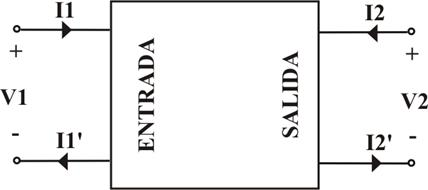
\includegraphics[width=0.6\textwidth]{imagen1.png}
		\caption{Un cuadripolo}
	\end{figure}

	Un ejemplo podría ser el siguiente circuito (figura \ref{cuadripolo_2}) 
	que está conformado por unos resistores, que forman dos mallas cuyas 
	corrientes entrantes y salientes son iguales; cumpliendo 
	todas las condiciones para ser considerado un cuadripolo.
	\begin{figure}[H]
		\centering
		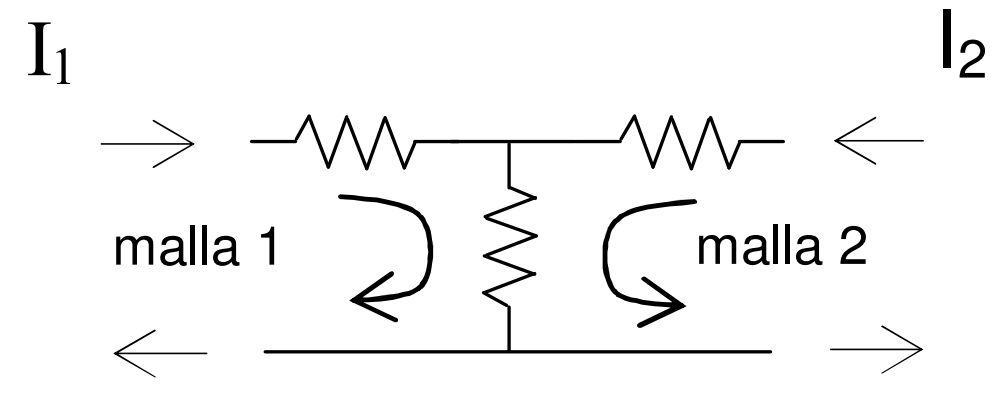
\includegraphics[width=0.6\textwidth]{imagen2.png}
		\caption{Otro cuadripolo}
		\label{cuadripolo_2}
	\end{figure}

	Existen dos grandes ramas para dividir a los cuadripolos; 
	por el lado de los lineales los podemos subdividir en activos 
	(con fuentes dependientes o independientes) o pasivos (recíprocos o simétricos).

	Los activos se caracterizan principalmente por poder llegar a entregar en la salida
	una potencia mayor que la que ingresa por la entrada.
	Deben requerir una fuente dependiente.

	En cambio, los pasivos, son aquellos que incluyen elementos que hacen que la potencia
	que egresa hacia la carga sea igual o inferior a la que ingresa, por ende, se disipa
	potencia dentro del circuito

	En cuanto al análisis hay una nomenclatura matemática denominada
	transferencia que enuncia como se relaciona la entrada con la salida
	del cuadripolo. 

	El ejemplo más simple como para entenderlo sería el de dos cables entre
	la entrada y salida, la relación entre la entrada y el factor de
	transferencia seria 1, que resultaría a la salida $Vo=Vi*1$

	\subsection{Inter-conexionado de cuadripolos}		
		\subsubsection{Paralelo}
		\begin{figure}[H]
			\centering
			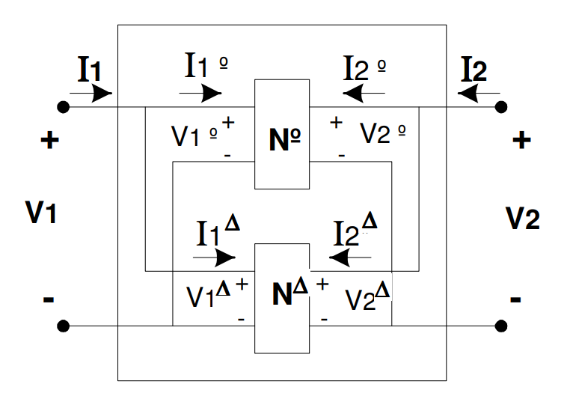
\includegraphics[width=\textwidth]{imagen3.png}
			\caption{Interconexion de cuadripolos en paralelo}
		\end{figure}
		En caso de tener dos cuadripolos interconectados, o desmembrar uno 
		más complejo en otros más simples, podemos generar cuatro situaciones;
		por un lado, si tenemos un Inter-conexionado en paralelo de dos cuadripolos.\\
		Ambos cuadripolos tienen tanto la misma tensión de entrada como de salida; 
		si queremos obtener un cuadripolo equivalente, es conveniente modelizarlos
		usando las tensiones como variables independientes, 
		utilizando el modelo de parámetros $Y$.

%		\[
%			\begin{bmatrix}
%				I^0_1 \\\\
%				I^0_2
%			\end{bmatrix}
%			=
%			\begin{bmatrix}
%				Y^0_{11} & Y^0_{12} \\\\
%				Y^0_{21} & Y^0_{22} 
%			\end{bmatrix} 
%			\begin{bmatrix}
%				V^0_1 \\\\\
%				V^0_2
%			\end{bmatrix}
%		\]
		\begin{figure}[H]
			\centering
			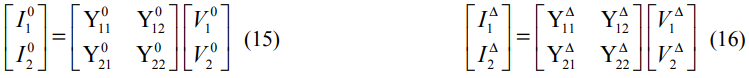
\includegraphics[width=0.8\textwidth]{imagen4.png}
		\end{figure}
		{\centering	{Concluyendo en que la matriz equivalente resultante es:}}
		\[
		\begin{bmatrix} Y \end{bmatrix} 
			=
		\begin{bmatrix} Y^0 \end{bmatrix} 
			+
		\begin{bmatrix} Y^{\Delta} \end{bmatrix} 
		\]
		(tener en cuenta que esto es valido si los bornes de acceso al
		cuadripolo equivalente son los pares de terminales de 
		cada uno de los cuadripolos)


		\subsubsection{Serie}
		\begin{figure}[H]
			\centering
			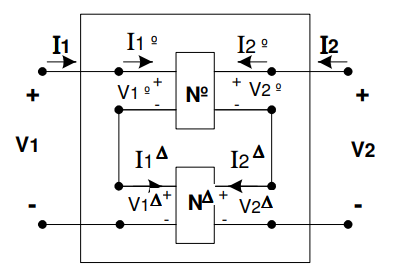
\includegraphics[width=\textwidth]{imagen5.png}
			\caption{Interconexion de cuadripolos en serie}
		\end{figure}
		En el caso de tener una interconexión resultante en serie, donde las
		corrientes de entrada y salida son iguales, y queremos obtener un 
		cuadripolo equivalente; calculamos a través del modelo en parámetros
		Z para cada uno. Obteniendo:
		\begin{figure}[H]
			\centering
			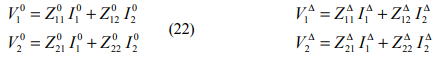
\includegraphics[width=0.8\textwidth]{imagen6.png}
		\end{figure}
		Luego obtener la función equivalente al cuadripolo resultante en
		función de Z; verificamos que la tensión resultante es igual a la
		suma de las dos anteriores, y que la corriente es igual a la de cada cuadripolo base.\\
		\(
			V_1 = Z_{11} \x I_{1}	+	Z_{12} \x I_{2} \\
			V_2 = Z_{21} \x I_{1}	+	Z_{22} \x I_{2} 
		\)
		Por lo que luego de reemplazar las ecuaciones concluimos que la matriz resultante es:
		\[
		\begin{bmatrix} Z \end{bmatrix} 
			=
		\begin{bmatrix} Z^0 \end{bmatrix} 
			+
		\begin{bmatrix} Z^{\Delta} \end{bmatrix} 
		\]

		\subsubsection{Cascada}
		\begin{figure}[H]
			\centering
			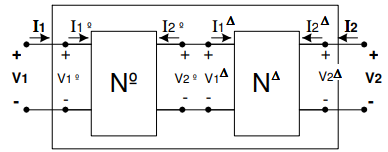
\includegraphics[width=\textwidth]{imagen7.png}
			\caption{Interconexion de cuadripolos en cascada}
		\end{figure}
		En el caso de la interconexión cascada, siendo esta la mas sencilla
		donde los bornes de salida de uno se conectan a los de entrada del
		otro cuadripolo. Dado que los valores de salida de uno son los de
		entrada del otro, lo mas inteligente es usar los parámetros T para
		analizar la conexión. Cosa que nos dará como conclusión
		
		\begin{figure}[H]
			\centering
			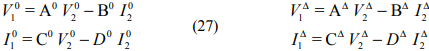
\includegraphics[width=0.8\textwidth]{imagen8.png}
		\end{figure}

		Y a su vez la matriz total equivalente es.
		\[
		\begin{bmatrix} T \end{bmatrix} 
			=
		\begin{bmatrix} T^0 \end{bmatrix} 
			\x
		\begin{bmatrix} T^{\Delta} \end{bmatrix} 
		\]

		\subsubsection{Mixto}
		\begin{figure}[H]
			\centering
			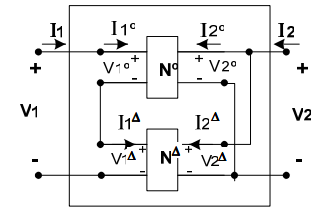
\includegraphics[width=\textwidth]{imagen9.png}
			\caption{Interconexion de cuadripolos de forma mixta}
		\end{figure}
		Como último caso se puede dar que tengamos una conexión mixta, esto quiere
		decir que un par de bornes se encuentran en una interconexión en serie,
		y el otro en paralelo o viceversa. Para solucionar este conexionado donde
		las tensiones de salida resultan en las corrientes de entrada, y las
		corrientes de salida en las tensiones de entrada; usaremos un sistema 
		mixto de parámetros $H$ y $H’$

		Para cada cuadripolo escribiremos:	
		\begin{figure}[H]
			\centering
			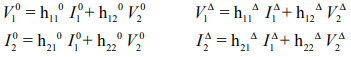
\includegraphics[width=0.8\textwidth]{imagen10.png}
		\end{figure}

		Luego de verificar que la tensión de entrada del cuadripolo equivalente
		es igual a la suma de las individuales, y que las corrientes de salida 
		son la suma de las corrientes individuales

		Reemplazamos las ecuaciones hasta llegar a 
		\(
		\begin{bmatrix} V_1 \\ I_2 \end{bmatrix} = [H] \begin{bmatrix} I_1 \\ V_2 \end{bmatrix}
		\text{donde}
		\begin{bmatrix} H \end{bmatrix} 
			=
		\begin{bmatrix} H^0 \end{bmatrix} 
			+
		\begin{bmatrix} H^{\Delta} \end{bmatrix} 
		\)


		\subsubsection{Cuadripolo Reciproco:}
		Un cuadripolo es recíproco cuando, conectado a sus puertos un generador de tensión y
		un amperímetro ideales (con resistencias internas despreciables), el intercambio de las
		posiciones del generador y del amperímetro, no producen ninguna alteración en el valor
		de la corriente que marca este último. La condición de reciprocidad puede ser definida
		también, de forma análoga, haciendo referencia a un generador de corriente y un 
		voltímetro ideales.
		}
		\subsubsection{Cuadripolo Simétrico:}
		En un cuadripolo simétrico, es indiferente conectar el generador y la carga en 
		cualquiera de sus puertos y los diferentes parámetros característicos verifican o 
		cumplen ciertas relaciones. Esto nos da a entender que un cuadripolo recíproco es 
		simétrico cuando el intercambio de las posiciones de sus puertos, entrada y salida,
		no producen ninguna alteración en las corrientes y tensiones de las mismas.

	{
	\renewcommand{\subsectionbreak}{}
	\subsection{Otras características}
	\begin{itemize}
    \item El Cuadripolo no contiene fuentes independientes de energía (Cuadripolo pasivo), 
		 pero puede contener fuentes dependientes (como en los circuitos equivalentes de dispositivos electrónicos). 
    \item  En ausencia de excitación externa no hay energía almacenada en el Cuadripolo. 
    \item  La corriente que sale por una puerta es igual a la que entra en la misma. 
    \item Las conexiones externas deben hacerse al puerto de entrada o al puerto de salida. 
    \item No se permiten conexiones externas entre los puertos.
	\end{itemize}
	}

\end{document}
